% Authors: Nelson Lago and Fernanda Magano
% This file is distributed under the MIT Licence

%%%%%%%%%%%%%%%%%%%%%%%%%%%%%%%%%%%%%%%%%%%%%%%%%%%%%%%%%%%%%%%%%%%%%%%%%%%%%%%%
%%%%%%%%%%%%%%%%%%%%%%%%%%%%%%%%% PREÂMBULO %%%%%%%%%%%%%%%%%%%%%%%%%%%%%%%%%%%%
%%%%%%%%%%%%%%%%%%%%%%%%%%%%%%%%%%%%%%%%%%%%%%%%%%%%%%%%%%%%%%%%%%%%%%%%%%%%%%%%

% aspectratio default é 4:3;
% as mais úteis são 169 (16:9), 1610 (16:10) e 149 (14:9)
% A língua padrão é a última citada
\documentclass[
  xcolor={hyperref,svgnames,x11names,table},
  hyperref={pdfencoding=unicode,plainpages=false,pdfpagelabels=true,breaklinks=true},
  brazilian,english,12pt,aspectratio=149,
]{beamer}

% Vários pacotes e opções de configuração genéricos
\usepackage{imegoodies}
\usepackage[slides,hidelinks]{imelooks}

% Diretórios onde estão as figuras; com isso, não é necessário (mas
% é permitido) colocar o caminho completo em \includegraphics. Note
% que a extensão nunca é necessária (mas é permitida), ou seja, o
% resultado é o mesmo com "\includegraphics{figuras/foto.jpeg}",
% "\includegraphics{foto.jpeg}", "\includegraphics{figuras/foto}"
% ou "\includegraphics{foto}".
\graphicspath{{figuras/},{fig/},{logos/},{img/},{images/},{imagens/}}

% Comandos rápidos para mudar de língua:
% \en -> muda para o inglês
% \br -> muda para o português
% \texten{blah} -> o texto "blah" é em inglês
% \textbr{blah} -> o texto "blah" é em português
\babeltags{br = brazilian, en = english}


%%%%%%%%%%%%%%%%%%%%%%%%%% COMANDOS PARA O USUÁRIO %%%%%%%%%%%%%%%%%%%%%%%%%%%%%

% A cada nova seção, recapitula o sumário.
% Para desabilitar, é só comentar este trecho
\AtBeginSection[]{
  \begin{frame}<beamer>[t]{Overview}
    \intermezzo
  \end{frame}
}

% Blocos de cor personalizada
\newenvironment{coloredblock}[2]%
  {
    \setbeamercolor{block title}{fg=white,bg=#1!80!white}
    \setbeamercolor{block body}{fg=darkgray,bg=#1!20!white}
    \setbeamercolor{local structure}{fg=darkgray,bg=#1!20!white}
    \begin{block}{#2}
  }
  {\end{block}}


%%%%%%%%%%%%%%%%%%%%%%%%%%%%%%%%%%%%%%%%%%%%%%%%%%%%%%%%%%%%%%%%%%%%%%%%%%%%%%%%
%%%%%%%%%%%%%%%%%%%%%%%%%% METADADOS E SLIDE TÍTULO %%%%%%%%%%%%%%%%%%%%%%%%%%%%
%%%%%%%%%%%%%%%%%%%%%%%%%%%%%%%%%%%%%%%%%%%%%%%%%%%%%%%%%%%%%%%%%%%%%%%%%%%%%%%%

% O arquivo com os dados bibliográficos para biblatex; você pode usar
% este comando mais de uma vez para acrescentar múltiplos arquivos
\addbibresource{bibliografia.bib}

\title[Percepções em Transformação]{Percepções em Transformação}

\subtitle{\normalsize Os impactos da IA generativa na produção de \emph{software}}

\author[Shortened Author Names]{Cássio Azevedo Cancio}

\institute{\textbf{Orientador:} Paulo Meirelles \\ \textbf{Coorientador:} Arthur Pilone}

\date{10 de dezembro de 2025}

% Coloca a imagem no fundo da página de título
\titlebgimage{\includegraphics[width=\paperwidth,height=\paperheight]%
             {bg-ime}}

% Logotipos no rodapé da página de título. Na verdade, qualquer coisa pode
% ser colocada aqui para aparecer próximo ao final da página de título.
% Esse material é colocado em uma minipage de largura .7\textwidth, porque
% o pano de fundo tem um pedaço muito escuro à direita da página.
%
% De acordo com o manual de identidade visual, a altura do logo da USP deve
% ser 2/3 da altura do logo do IME; o logo da USP deve ficar deslocado para
% cima 1/6 da altura do logo do IME. As posições e tamanhos dos logos da
% fapesp/capes/cnpq não seguem nenhuma lógica bem definida (na verdade,
% nada está alinhado com nada!): eu (Nelson) fiz "a olho" da maneira que
% me pareceu mais harmônica.
\logos{%
  \includegraphics[height=.9\baselineskip]{ime-logo}%
  \quad\quad
  \raisebox{.15\baselineskip}{\includegraphics[height=.6\baselineskip]{usp-logo}}%
  %\quad\quad
  %\raisebox{.178\baselineskip}{\includegraphics[height=.515\baselineskip]{fapesp-logo}}%
  %\quad\quad
  %\raisebox{-.1732\baselineskip}{\includegraphics[height=1.2\baselineskip]{capes-logo}}%
  %\quad\quad
  %\raisebox{.124\baselineskip}{\includegraphics[height=.6\baselineskip]{cnpq-logo}}%
  \par
  % Queremos que o logo cc-by fique próximo da margem direita da página, mas
  % este material está dentro de uma minipage de largura .7\textwidth. Assim,
  % usamos esse hspace, que "estoura" a largura da minipage para a direita.
  \hspace{.87\paperwidth}\includegraphics[width=.05\paperwidth]{cc-by}\par
}

% Usado para criar o qrcode com o endereço da apresentação
\qrcodeurl{https://cassiocancio.github.io/TCC-BCC/}

% Inclui ou não o qrcode no sumário da apresentação
%\qrcodeintoc % default
%\noqrcodeintoc

% O slide de sumário pode ser dividido em colunas; o parâmetro
% determina após qual o número da seção fazer a quebra de coluna
% (use zero para uma coluna ou simplesmente omita este comando).
\toccolumnsplit{5}


%%%%%%%%%%%%%%%%%%%%%%%%%%%%%%%%%%%%%%%%%%%%%%%%%%%%%%%%%%%%%%%%%%%%%%%%%%%%%%%%
%%%%%%%%%%%%%%%%%%%%%%%%%%%% INÍCIO DA APRESENTAÇÃO %%%%%%%%%%%%%%%%%%%%%%%%%%%%
%%%%%%%%%%%%%%%%%%%%%%%%%%%%%%%%%%%%%%%%%%%%%%%%%%%%%%%%%%%%%%%%%%%%%%%%%%%%%%%%

\begin{document}

\maketitle

\small

\section{Introdução}

\subsection{Contexto}

\begin{frame}{Contexto}
  - Popularização dos computadores e celulares;

  - Disparada no crescimento de sistemas de \emph{software} nas últimas décadas;

  - Muitos dados gerados e disponíveis para treinamento de modelos de IA;

  - GitHub Copilot e ChatGPT são lançados em 2022.
\end{frame}

\subsection{Objetivo}

\begin{frame}{Objetivo}
  - Levantar dados sobre os impactos da IA generativa na produção de \emph{software};

  - Analisar a evolução da percepção dos desenvolvedores sobre IA;

  - Comparar resultados de diferentes fontes da literatura cinza e formal.
\end{frame}

% -------------------------
\section{Ferramentas de IA}
\subsection{Uso entre desenvolvedores}
\begin{frame}{\insertsubsectionhead}
  \vspace{0.1cm}
  \centering
  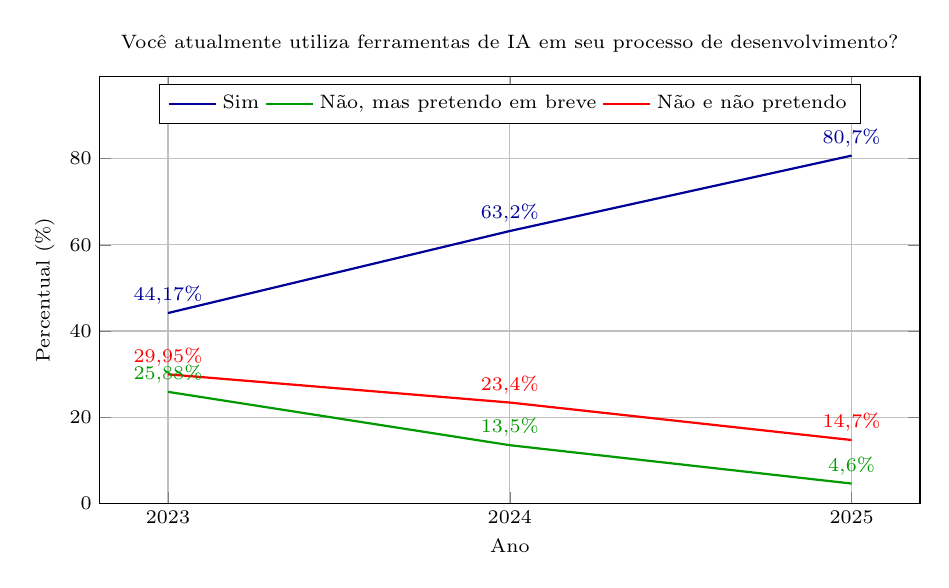
\begin{tikzpicture}
    \scriptsize
    \begin{axis}[
        /pgf/number format/use comma,
        width=12cm,
        height=7cm,
        title={Você atualmente utiliza ferramentas de IA em seu processo de desenvolvimento?},
        xlabel={Ano},
        ylabel={Percentual (\%)},
        ymin=0, ymax=99,
        symbolic x coords={2023,2024,2025},
        xtick=data,
        legend pos=south east,
        legend cell align={left},
        legend style={
            font=\scriptsize,
            at={(0.5,0.89)},
            anchor=south,
            legend columns=5,
          },
        grid=both,
        nodes near coords={\pgfmathprintnumber{\pgfplotspointmeta}\%},
        every axis plot/.style={ line width=1.5pt },
      ]

      % Yes (green)
      \addplot[
        thick,
        color=blue!60!black
      ] coordinates {
          (2023,44.17)
          (2024,63.2)
          (2025,80.7)
        };
      \addlegendentry{Sim}

      % No, but I plan to soon (orange)
      \addplot[
        thick,
        color=green!60!black
      ] coordinates {
          (2023,25.88)
          (2024,13.5)
          (2025,4.6)
        };
      \addlegendentry{Não, mas pretendo em breve}

      % No, and I don't plan to (red)
      \addplot[
        thick,
        color=red
      ] coordinates {
          (2023,29.95)
          (2024,23.4)
          (2025,14.7)
        };
      \addlegendentry{Não e não pretendo}

    \end{axis}
  \end{tikzpicture}

  \vspace{-0.25cm}

  \footnotesize
  \cite{StackOverflow2023,StackOverflow2024,StackOverflow2025}
\end{frame}

\subsection{Previsões sobre o uso}
\begin{frame}{\insertsubsectionhead}
  Segundo previsões da \emph{Gartner Research} (\cite{gartner_ai_code_assistants_2024}):

  \vspace{0.5cm}

  - Em 2028, 90\% das empresas de \emph{software} usarão \emph{AI code assistants}.

  - O ciclo de desenvolvimento passará de 5\% (2024) para 40\% (2027) feito por IA.

  - Até 2027, 25\% dos bugs em produção virão de \textbf{código de IA não revisado}.

\end{frame}

\subsection{Casos de uso}
\begin{frame}{\insertsubsectionhead}
  De acordo com \cite{elsevier}, desenvolvedores preferem:

  - \textbf{Delegar tarefas menos prazerosas} para ferramentas de IA.

  - \textbf{Manter controle} das atividades mais interessantes.

  \vspace{0.4cm}
  \centering
  \begin{tabular}{p{5 cm}p{3cm}p{3cm}}
    Atividade                   & Delegaria                 & Gosta de fazer            \\
    \toprule

    Escrita de testes           & \cellcolor{green!10} 70\% & \cellcolor{red!10} 30\%   \\
    Documentação técnica        & \cellcolor{green!10} 66\% & \cellcolor{red!10} 26\%   \\
    Criar novas \emph{features} & \cellcolor{red!10} 27\%   & \cellcolor{green!10} 86\% \\
  \end{tabular}
\end{frame}

\begin{frame}{\insertsubsectionhead}
  Segundo \cite{StackOverflow2024}, dentre os profissionais que usam IA:

  \vspace{0.5cm}

  - 82\% usa IA para \textbf{escrever código}.

  - 40,1\% para \textbf{produzir documentação}.

  - 27,2\% para \textbf{testar código}.
\end{frame}

\section{Análise de métricas}

\subsection{Tabela de métricas}
\begin{frame}{\insertsubsectionhead}

  \vspace{0.5cm}

  - A \cite{gitclear2025} analisou \textbf{211 milhões de linhas de código} em 2025.

  - O código tem origem em milhares de empresas e repositórios de código aberto.

  - O relatório compila as métricas de 2020 a 2024.

  \begin{center}
    \footnotesize
    \begin{tabular}{p{0.8cm}p{1.8cm}p{1.8cm}p{1.8cm}p{1.8cm}p{1.8cm}}
      \toprule
      Ano  & Adicionada                  & Movida                    & Copiada                   & Substituída                & Churn                    \\
      \toprule
      2020 & 39,2\%                      & 24,1\%                    & 8,3\%                     & 2,9\%                      & 3,1\%                    \\

      2021 & 39,5\%                      & 24,8\%                    & 8,4\%                     & 3,4\%                      & 3,3\%                    \\

      2022 & 40,9\%                      & \cellcolor{red!10} 20,5\% & 9,4\%                     & 3,7\%                      & 3,3\%                    \\

      2023 & \cellcolor{green!15} 42,3\% & \cellcolor{red!20} 15,8\% & \cellcolor{red!10} 10,6\% & \cellcolor{green!10} 3,6\% & \cellcolor{red!10} 4,5\% \\

      2024 & \cellcolor{green!30} 46,2\% & \cellcolor{red!40} 9,5\%  & \cellcolor{red!20} 12,3\% & \cellcolor{green!20} 4,2\% & \cellcolor{red!20} 5,7\% \\

    \end{tabular}

  \end{center}

\end{frame}

\subsection{Principais resultados}
\begin{frame}{\insertsubsectionhead}
  \footnotesize

  \textbf{Queda na refatoração}

  - A \% de \textbf{linhas movidas}, indicador de refatoração, caiu de 24,1\% (2020) para 9,5\% (2024).

  \vspace{0.25cm}
  
  \textbf{Aumento de duplicações:}
  
  - Em 2024, pela 1ª vez, a \% de \textbf{linhas copiadas (12,3\%) superou as linhas movidas (9,5\%)}.
  
  - A ocorrência de commits com \textbf{código duplicados} foi de 0,7\% (2020) para 6,66\% (2024).

  \vspace{0.25cm}
  
  \textbf{Aumento do retrabalho (churn):}
  
  - O churn cresceu de 3,1\% em 2020 para 5,7\% em 2024.
\end{frame}

\begin{frame}{\insertsubsectionhead}
  \vspace{0.25cm}
  \centering
  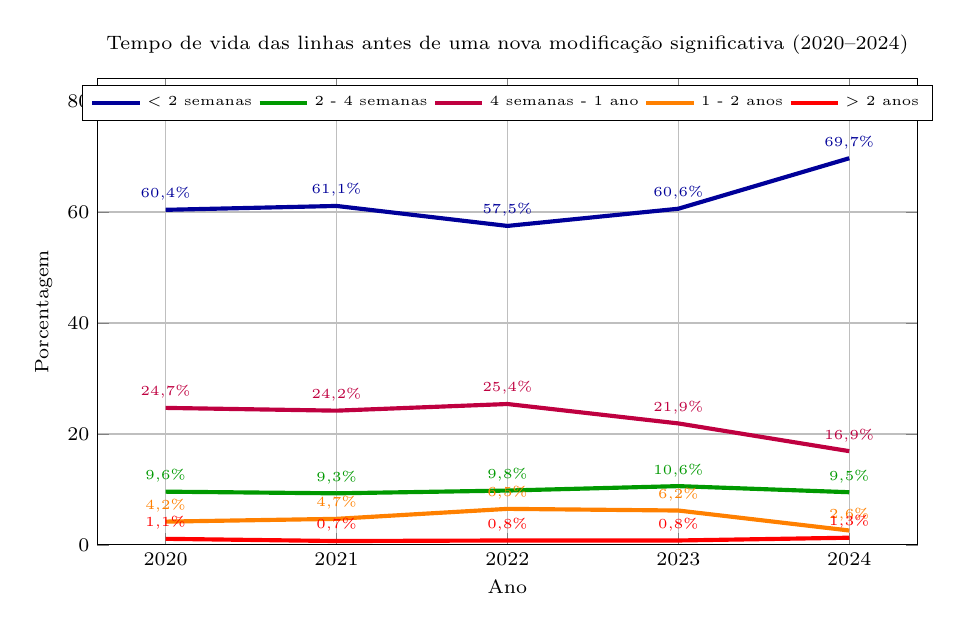
\begin{tikzpicture}
    \scriptsize
    \begin{axis}[
        /pgf/number format/use comma,
        every axis plot/.style={ line width=1.5pt },
        width=12cm,
        height=7.5cm,
        xlabel={Ano},
        ylabel={Porcentagem},
        title={Tempo de vida das linhas antes de uma nova modificação significativa (2020–2024)
          },
        ymin=0,
        ymax=84,
        legend style={
            font=\tiny,
            at={(0.5,0.91)},
            anchor=south,
            legend columns=5,
          },
        grid=both,
        symbolic x coords={2020,2021,2022,2023,2024},
        xtick=data,
        nodes near coords={\pgfmathprintnumber{\pgfplotspointmeta}\%},
        every node near coord/.append style={
            font=\tiny,
            anchor=south,
          },
      ]

      \addplot[color=blue!60!black] coordinates {
          (2020,60.4) (2021,61.1) (2022,57.5) (2023,60.6) (2024,69.7)
        };
      \addlegendentry{< 2 semanas}

      \addplot[color=green!60!black] coordinates {
          (2020,9.6) (2021,9.3) (2022,9.8) (2023,10.6) (2024,9.5)
        };
      \addlegendentry{2 - 4 semanas}

      \addplot[color=purple] coordinates {
          (2020,24.7) (2021,24.2) (2022,25.4) (2023,21.9) (2024,16.9)
        };
      \addlegendentry{4 semanas - 1 ano}

      \addplot[color=orange] coordinates {
          (2020,4.2) (2021,4.7) (2022,6.5) (2023,6.2) (2024,2.6)
        };
      \addlegendentry{1 - 2 anos}

      \addplot[color=red] coordinates {
          (2020,1.1) (2021,0.7) (2022,0.8) (2023,0.8) (2024,1.3)
        };
      \addlegendentry{> 2 anos}

    \end{axis}
  \end{tikzpicture}

\end{frame}

\section{Referências}

\begin{frame}[allowframebreaks]{Referências}
  \nocite{anssi_2024,StackOverflow2023,StackOverflow2024,StackOverflow2025,elsevier,gitclear2025,gartner_ai_code_assistants_2024}
  \printbibliography
\end{frame}

% Slides do tipo "Fim" ou "Perguntas?" não são muito úteis; ao invés
% disso, é mais interessante definir um slide final recapitulando o
% que foi visto.
\begin{frame}[t]{\insertshorttitle}
  \overview

  % \begin{center} acrescenta espaço vertical; como possivelmente temos
  % pouco espaço aqui, vamos usar centering e adicionar o espaço manualmente
  \vspace{1\baselineskip}
  \bgroup
  \centering
  \url{https://cassiocancio.github.io/TCC-BCC/}\par
  \egroup

\end{frame}

\end{document}
